\subsubsection{ Digit readers }

\begin{itemize}

\item For each $i = 1,2,3$,
               $j = l-1,\ldots,1$,
               $u \in \{0, 1\}^j$, and
               $\inc \in \{{\tt increment}, {\tt copy} \}$:
    \begin{itemize}
        \item if $j = 0$:
        create
        $\begin{aligned}[t]
            \dreader(& \left\langle {\tt DigitReader}, i, \lambda, \inc \right\rangle, \\
                     & \left\langle {\tt DigitReader}, i, 0, \inc \right\rangle, \\
                     & \left\langle {\tt DigitReader}, i, 1, \inc \right\rangle \;)
        \end{aligned}$\\ from the general gadget in Figure~\ref{fig:digit_read}

        \item if $1 \leqslant j \leqslant l -2$:
        create
        $\begin{aligned}[t]
        \dreader(& \left\langle {\tt DigitReader}, i, u,  \inc \right\rangle, \\
                 & \left\langle {\tt DigitReader}, i, 0u, \inc \right\rangle, \\
                 & \left\langle {\tt DigitReader}, i, 1u, \inc \right\rangle \;)
        \end{aligned}$\\ from the general gadget in Figure~\ref{fig:digit_read}

        \item if $j = l - 1$:
        create
        $\begin{aligned}[t]
            \dreader(& \left\langle {\tt DigitReader}, i, u, \inc \right\rangle, \\
                     & \left\langle {\tt PreWarp}, i, 0u, \inc \right\rangle, \\
                     & \left\langle {\tt PreWarp}, i, 1u, \inc \right\rangle \;)
        \end{aligned}$\\from the general gadget in Figure~\ref{fig:digit_read}

    \end{itemize}


\end{itemize}

\begin{figure}[H]
    \centering
    \begin{subfigure}[t]{0.2\textwidth}
        \centering
        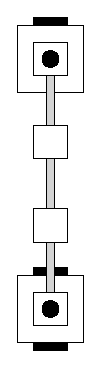
\includegraphics[width=0.2\textwidth]{read/read_0}
        \caption{\label{fig:read_0} {\tt Read\_0}}
    \end{subfigure}%
    ~
    \begin{subfigure}[t]{0.2\textwidth}
        \centering
        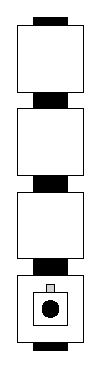
\includegraphics[width=0.2\textwidth]{read/read_1}
        \caption{\label{fig:read_1} {\tt Read\_1}}
    \end{subfigure}%
    \caption{\label{fig:digit_read} {\tt Read} gadgets}
\end{figure}
